\documentclass[14pt]{beamer}
\usepackage{./Estilos/BeamerUVM}
\usepackage{./Estilos/ColoresLatex}
\usetheme{Madrid}
\usecolortheme{default}
%\useoutertheme{default}
\setbeamercovered{invisible}
% or whatever (possibly just delete it)
\setbeamertemplate{section in toc}[sections numbered]
\setbeamertemplate{subsection in toc}[subsections numbered]
\setbeamertemplate{subsection in toc}{\leavevmode\leftskip=3.2em\rlap{\hskip-2em\inserttocsectionnumber.\inserttocsubsectionnumber}\inserttocsubsection\par}
% \setbeamercolor{section in toc}{fg=blue}
% \setbeamercolor{subsection in toc}{fg=blue}
% \setbeamercolor{frametitle}{fg=blue}
\setbeamertemplate{caption}[numbered]

\setbeamertemplate{footline}
\beamertemplatenavigationsymbolsempty
\setbeamertemplate{headline}{}


\makeatletter
% \setbeamercolor{section in foot}{bg=gray!30, fg=black!90!orange}
% \setbeamercolor{subsection in foot}{bg=blue!30}
% \setbeamercolor{date in foot}{bg=black}
\setbeamertemplate{footline}
{
  \leavevmode%
  \hbox{%
  \begin{beamercolorbox}[wd=.333333\paperwidth,ht=2.25ex,dp=1ex,center]{section in foot}%
    \usebeamerfont{section in foot} {\insertsection}
  \end{beamercolorbox}%
  \begin{beamercolorbox}[wd=.333333\paperwidth,ht=2.25ex,dp=1ex,center]{subsection in foot}%
    \usebeamerfont{subsection in foot}  \insertsubsection
  \end{beamercolorbox}%
  \begin{beamercolorbox}[wd=.333333\paperwidth,ht=2.25ex,dp=1ex,right]{date in head/foot}%
    \usebeamerfont{date in head/foot} \insertshortdate{} \hspace*{2em}
    \insertframenumber{} / \inserttotalframenumber \hspace*{2ex} 
  \end{beamercolorbox}}%
  \vskip0pt%
}
\makeatother

\makeatletter
\patchcmd{\beamer@sectionintoc}{\vskip1.5em}{\vskip0.8em}{}{}
\makeatother

% \usefonttheme{serif}
\usepackage[clock]{ifsym}
\usetikzlibrary{plotmarks}
\usepackage[version=4]{mhchem}

\sisetup{per-mode=symbol}
\resetcounteronoverlays{saveenumi}
\DeclareSIUnit[number-unit-product = {\,}]\cal{cal}

% \newcommand{\nsum}[1][1.4]{% only for \displaystyle
%     \mathop{%
%         \raisebox
%             {-#1\depthofsumsign+1\depthofsumsign}
%             {\scalebox
%                 {#1}
%                 {$\displaystyle\sum$}%
%             }
%     }
% }

\title{\Large{Magnetismo} \\ \normalsize{Física 2}}
\date{8 de agosto de 2023}

\begin{document}
\maketitle

\section*{Contenido}
\frame{\frametitle{Contenido} \tableofcontents[currentsection, hideallsubsections]}

\section{Magnetismo}
\frame{\tableofcontents[currentsection, hideothersubsections]}
\subsection{Introducción}

\begin{frame}
\frametitle{Relato inicial}
Hace dos mil años aproximadamente, unos pastores de Magnesia (ciudad antigua de Turquía), \pause cuando conducían a sus corderos a cierto pasto, sintieron una fuerte atracción hacia el suelo debido a la punta metálica de su bastón y a los clavos de su calzado, que les dificultó seguir caminando.
\end{frame}
\begin{frame}
\frametitle{Magnesia}
\begin{figure}
    \centering
    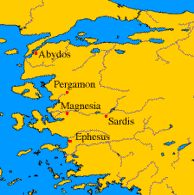
\includegraphics[scale=0.65]{Imagenes/Magnetismo_01.png}
\end{figure}
\end{frame}
\begin{frame}
\frametitle{Relato inicial}    
Interesados por encontrar la causa removieron la tierra y descubrieron una roca negra, la cual atraía al hierro.
\\
\bigskip
\pause
Hoy esta roca recibe el nombre de \textocolor{blue-violet}{piedra imán} o \textocolor{blue-violet}{magnetita}; \pause  químicamente es un mineral de óxido de hierro cuya fórmula es \ce{Fe3O4}.
\end{frame}
\begin{frame}
\frametitle{La piedra imán}
\begin{figure}
    \centering
    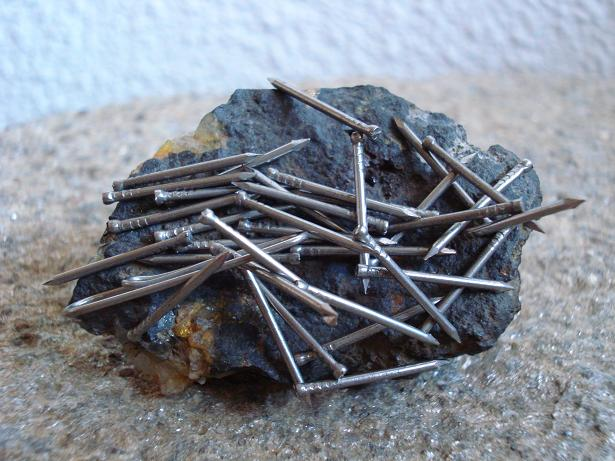
\includegraphics[scale=0.5]{Imagenes/Magnetismo_02.jpg}
\end{figure}
\end{frame}
\begin{frame}
\frametitle{Estudios con imanes}
William Gilbert científico inglés, demostró con sus experimentos que \textocolor{cobalt}{la Tierra se comporta como un imán enorme}, por tanto obliga a un extremo de la brújula a apuntar al Norte magnético.
\end{frame}
\begin{frame}
\frametitle{Estudios con imanes}    
También demostró que cuando un imán se rompe en varios pedazos, cada uno se transforma en uno nuevo con sus \textocolor{darkolivegreen}{dos polos} en cada extremo.
\end{frame}
\begin{frame}
\frametitle{Propiedad de los imanes}
Gilbert descubrió cómo interactúan los polos de los imanes y demostró que \textocolor{red}{polos iguales} se rechazan \pause y \textocolor{cadetblue}{polos distintos} se atraen.
\end{frame}
\begin{frame}
\frametitle{Más estudios con los imanes}
Posteriormente el científico inglés Michael Faraday estudió los efectos producidos por los imanes.
\end{frame}
\begin{frame}
\frametitle{Más estudios con los imanes}    
Observó que un imán permanente ejerce una fuerza sobre un trozo de hierro o sobre cualquier imán cercano a él, \pause debido a la presencia de un \textocolor{amethyst}{campo de fuerzas} cuyos efectos se hacen sentir incluso a través de un espacio vacío.
\end{frame}
\begin{frame}
\frametitle{Más estudios con los imanes}    
Faraday imaginó que de un imán salían hilos o líneas que se esparcían, \pause a éstas las llamó \textocolor{ao(english)}{líneas de fuerza magnética}.
\\
\bigskip
\pause
Dichas líneas se encuentran más en los polos pues ahí la intensidad es mayor.
\end{frame}
\begin{frame}
\frametitle{Líneas de fuerza magnética}
\begin{figure}
    \centering
    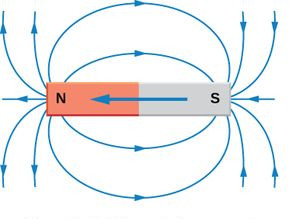
\includegraphics[scale=1]{Imagenes/Magnetismo_03a.jpg}
\end{figure}
\end{frame}
\begin{frame}
\frametitle{Líneas de fuerza magnética}
\begin{figure}
    \centering
    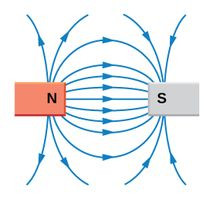
\includegraphics[scale=1]{Imagenes/Magnetismo_03b.jpg}
\end{figure}
\end{frame}
\begin{frame}
\frametitle{Líneas de fuerza magnética}
\begin{figure}
    \centering
    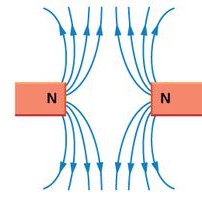
\includegraphics[scale=1]{Imagenes/Magnetismo_03c.jpg}
\end{figure}
\end{frame}
\begin{frame}
\frametitle{El campo magnético}
A la zona que rodea a un imán y en la cual su influencia puede detectarse recibe el nombre de \textocolor{bulgarianrose}{campo magnético}.
\end{frame}
\begin{frame}
\frametitle{El campo magnético}
Faraday señaló que cuando dos imanes se encuentran cerca uno de otro, sus campos magnéticos se interfieren recíprocamente.
\end{frame}

\subsection{Densidad de flujo magnético}

\begin{frame}
\frametitle{El concepto de flujo magnético}
El concepto propuesto por Faraday acerca de las líneas de fuerza es imaginario, pero resulta muy útil para dibujar los campos magnéticos y cuantificar sus efectos.
\end{frame}
\begin{frame}
\frametitle{El concepto de flujo magnético}
Una sola línea de fuerza equivale a la unidad de flujo magnético $\phi$ en el sistema CGS y recibe el nombre de \textocolor{carmine}{maxwell}.
\end{frame}
\begin{frame}
\frametitle{El concepto de flujo magnético}
Sin embargo, el \textocolor{carmine}{maxwell} es una unidad muy pequeña de flujo magnético, \pause por lo que en el Sistema Internacional se emplea una unidad mucho mayor llamada \textocolor{carminered}{weber}.
\end{frame}
\begin{frame}
\frametitle{El concepto de flujo magnético}
Un flujo magnético $\phi$ que atraviesa perpendicularmente una unidad de área $A$ recibe el nombre de \textocolor{carminepink}{densidad de flujo magnético} o \textocolor{carnelian}{inducción magnética} $B$.
\end{frame}
\begin{frame}
\frametitle{El concepto de flujo magnético}
Por definición: la densidad del flujo magnético en una región de un campo magnético equivale al número de líneas de fuerza (o sea al flujo magnético) que atraviesan perpendicularmente a la unidad de área.
\end{frame}
\begin{frame}
\frametitle{El concepto de flujo magnético}
Matemáticamente se expresa:
\pause
\begin{align*}
B = \dfrac{\phi}{A}
\end{align*}
donde:
\setbeamercolor{item projected}{bg=carrotorange,fg=black}
\setbeamertemplate{enumerate items}{%
\usebeamercolor[bg]{item projected}%
\raisebox{1.5pt}{\colorbox{bg}{\color{fg}\footnotesize\insertenumlabel}}%
}
\begin{enumerate}[<+->]
\item $B$ = densidad del flujo magnético, en el SI se mide en webers/metro cuadrado (Wb/\unit{\square\meter})
\seti
\end{enumerate}
\end{frame}
\begin{frame}
\frametitle{El concepto de flujo magnético}
\setbeamercolor{item projected}{bg=carrotorange,fg=black}
\setbeamertemplate{enumerate items}{%
\usebeamercolor[bg]{item projected}%
\raisebox{1.5pt}{\colorbox{bg}{\color{fg}\footnotesize\insertenumlabel}}%
}
\begin{enumerate}[<+->]
\conti
\item $\phi$ = flujo magnético, su unidad es el weber (Wb)
\item $A$ = área sobre la que actúa el flujo magnético, se expresa en metros cuadrados (\unit{\square\meter})
\end{enumerate}
\end{frame}
\begin{frame}
\frametitle{Otro nombre para la densidad de flujo}
La densidad del flujo magnético también recibe el nombre de \textocolor{cerulean}{inducción magnética}.
\end{frame}
\begin{frame}
\frametitle{Unidades del flujo magnético}
En el SI la unidad de densidad del flujo magnético es el Wb/m2, el cual recibe el nombre de \textocolor{cinnabar}{tesla} (\unit{\tesla}) en honor del físico yugoslavo Nicolás Tesla.
\end{frame}

\section{Electromagnetismo}
\frame{\tableofcontents[currentsection, hideothersubsections]}
\subsection{La relación entre dos áreas}

\begin{frame}
\frametitle{Definición}
La parte de la Física encargada de estudiar al conjunto de fenómenos que resultan de las acciones mutuas entre las \textocolor{burgundy}{corrientes eléctricas} y el \textocolor{cerise}{magnetismo}, recibe el nombre de \textocolor{cobalt}{electromagnetismo}.
\end{frame}
\begin{frame}
\frametitle{Contribuciones importantes}
El electromagnetismo tuvo su origen en el invento de la \textocolor{cadmiumred}{pila eléctrica} realizado por el italiano \textocolor{antiquefuchsia}{Alessandro Volta} en 1800.
\end{frame}
\begin{frame}
\frametitle{Contribuciones importantes}
Mientras el físico danés \textocolor{auburn}{Hans Christian Oersted} impartía una clase de Física a sus alumnos, \pause empujó en forma accidental una brújula que se encontraba bajo un alambre conectado a una pila, \pause el cual conducía una corriente eléctrica continua o directa.
\end{frame}
\begin{frame}
\frametitle{Contribuciones importantes}
Oersted observó con asombro cómo la aguja realizaba un giro de \ang{90} para colocarse perpendicularmente al alambre.
\pause
\begin{figure}
    \centering
    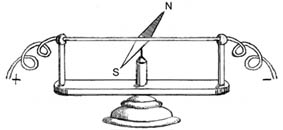
\includegraphics[scale=0.8]{Imagenes/Electromagnetismo_01.jpg}
\end{figure}
\end{frame}
\begin{frame}
\frametitle{Contribuciones importantes}
Con ello se demostraba que éste, además de conducir electricidad, generaba a su alrededor una fuerza parecida a la de un imán, \pause es decir, generaba un \textocolor{ao}{campo magnético}; \pause así se descubrió el \textocolor{blue(pigment)}{electromagnetismo}.
\end{frame}
\begin{frame}
\frametitle{Contribuciones importantes}    
Poco tiempo después, el científico francés \textocolor{bole}{André Marie Ampere}, descubrió que el campo magnético podía \textocolor{blush}{intensificarse} al enrollar el alambre conductor en forma de bobina.
\end{frame}
\begin{frame}
\frametitle{Contribuciones importantes}    
\begin{figure}
    \centering
    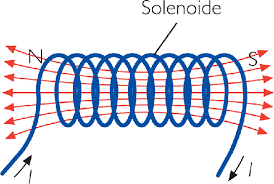
\includegraphics[scale=0.7]{Imagenes/Electromagnetismo_02.jpg}
\end{figure}
\end{frame}
\begin{frame}
\frametitle{Contribuciones importantes}
Este hecho condujo a \textocolor{carmine}{Joseph Henry}, a realizar otro descubrimiento importante: \pause se le ocurrió recubrir con un material aislante a un alambre y lo enrolló alrededor de una barra de hierro en forma de U.
\end{frame}
\begin{frame}
\frametitle{Contribuciones importantes}    
\begin{figure}
    \centering
    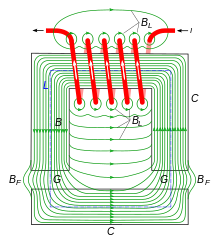
\includegraphics[scale=0.8]{Imagenes/Electromagnetismo_03.png}
\end{figure}
\end{frame}
\begin{frame}
\frametitle{Contribuciones importantes}
Luego, conectó los extremos del alambre a una batería y observó que la corriente eléctrica magnetizaba al hierro y cuando la corriente dejaba de circular entonces desaparecía el campo magnético de la barra de hierro.
\\
\bigskip
\pause
Se había descubierto el \textocolor{chestnut}{electroimán}, pieza fundamental de los motores eléctricos.
\end{frame}
\begin{frame}
\frametitle{Contribuciones importantes}
\begin{figure}
    \centering
    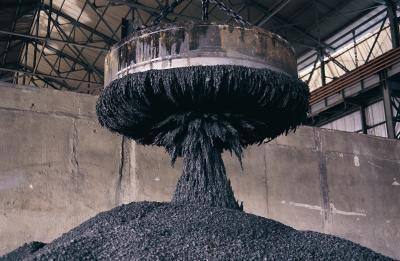
\includegraphics[scale=0.8]{Imagenes/Electromagnetismo_04.jpg}
\end{figure}
\end{frame}

\section{Campo magnético y corriente}
\frame{\tableofcontents[currentsection, hideothersubsections]}
\subsection{Conductor recto}

\begin{frame}
\frametitle{Regla de Ampere}
La \textocolor{burgundy}{regla de Ampere} señala que el polo norte de la aguja imantada se desvía siempre hacia la izquierda de la dirección de la corriente.
\end{frame}
\begin{frame}
\frametitle{Regla de Ampere}
\begin{figure}
    \centering
    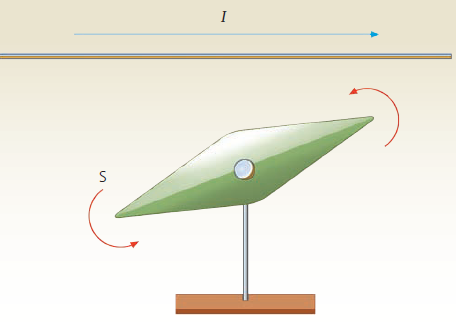
\includegraphics[scale=0.6]{Imagenes/Electromagnetismo_05.png}
\end{figure}
\end{frame}
\begin{frame}
\frametitle{Estudiando el campo magnético}
Para estudiar cómo es el campo magnético producido por un conductor recto en el cual circula una corriente eléctrica, hagamos lo siguiente:
\\
\bigskip
\pause
En un conductor rectilíneo colocamos un cartón horizontal rígido.
\end{frame}
\begin{frame}
\frametitle{Estudiando el campo magnético}
En el momento en que circula la corriente por el conductor, se espolvorea al cartón con limaduras de hierro y
se observa que éstas forman circunferencias concéntricas con el alambre.
\end{frame}
\begin{frame}
\frametitle{Estudiando el campo magnético}
\begin{figure}
    \centering
    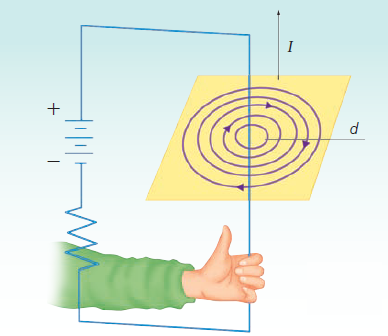
\includegraphics[scale=0.6]{Imagenes/Electromagnetismo_06.png}
\end{figure}
\end{frame}
\begin{frame}
\frametitle{Usando la regla de Ampere}
La regla de Ampere nos señala el sentido de las líneas de fuerza, pero también podemos aplicar \textocolor{red}{la regla de la mano izquierda}:
\end{frame}
\begin{frame}
\frametitle{Regla de la mano izquierda}
Como la dirección del \textocolor{cerise}{campo magnético} depende del sentido de la \textocolor{cadmiumred}{corriente}, \pause se toma al conductor recto con la mano izquierda con el pulgar extendido sobre el conductor.
\end{frame}
\begin{frame}
\frametitle{Regla de la mano izquierda}
El conductor debe señalar el sentido en el que circula la corriente eléctrica (de negativo a positivo) y
los cuatro dedos restantes indicarán el sentido del campo magnético.
\end{frame}
\begin{frame}
\frametitle{Regla de la mano izquierda}
\begin{figure}
    \centering
    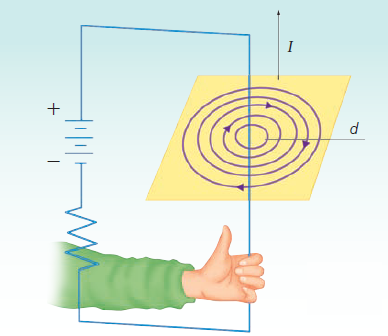
\includegraphics[scale=0.6]{Imagenes/Electromagnetismo_06.png}
\end{figure}
\end{frame}
\begin{frame}
\frametitle{Expresión para la inducción magnética}
Para determinar la \textocolor{byzantine}{inducción magnética} o \textocolor{byzantium}{densidad de flujo
magnético} ($\vb{B}$) \pause a una cierta \textocolor{blue}{distancia} $d$ de un conductor recto \pause por el que circula una \textocolor{carmine}{intensidad de corriente} $I$, se aplica la siguiente expresión matemática:
\end{frame}
\begin{frame}
\frametitle{Expresión para la inducción magnética}
\begin{align*}
B = \dfrac{\mu \, I}{2 \, \pi \, d}
\end{align*}
donde:
\setbeamercolor{item projected}{bg=aquamarine,fg=black}
\setbeamertemplate{enumerate items}{%
\usebeamercolor[bg]{item projected}%
\raisebox{1.5pt}{\colorbox{bg}{\color{fg}\footnotesize\insertenumlabel}}%
}
\begin{enumerate}[<+->]
\item $B$ es la inducción magnética, medida en teslas (T)
\item $\mu$ es la \textocolor{bronze}{permeabilidad} del medio que rodea al conductor, se expresa en $T \, m/A$
\seti
\end{enumerate}
\end{frame}
\begin{frame}
\frametitle{Expresión para la inducción magnética}
\begin{align*}
B = \dfrac{\mu \, I}{2 \, \pi \, d}
\end{align*}
\setbeamercolor{item projected}{bg=aquamarine,fg=black}
\setbeamertemplate{enumerate items}{%
\usebeamercolor[bg]{item projected}%
\raisebox{1.5pt}{\colorbox{bg}{\color{fg}\footnotesize\insertenumlabel}}%
}
\begin{enumerate}[<+->]    
\conti
\item $I$ es la corriente, medidad en Ampere (A)
\item $d$ es la distancia perpendicular entre el conductor y el punto considerado, medido en metros (m).
\end{enumerate}
\end{frame}
\begin{frame}
\frametitle{Permeabilidad en el vacío}
En el caso de que el medio que rodea al conductor es el vacío, se tiene que:
\pause
\begin{align*}
\mu = \mu_{0} = 4 \, \pi \times 10^{-7} \unit{\tesla\meter\per\ampere}
\end{align*}
\end{frame}

\subsection{Una espira}

\begin{frame}
\frametitle{Definiendo una espira}
Una \textocolor{cardinal}{espira} se obtiene al doblar en forma circular un conductor recto.
\end{frame}
\begin{frame}
\frametitle{El campo magnético en una espira}
El espectro del campo magnético creado por ésta, se origina por líneas cerradas que rodean a la corriente
y por una línea recta que es el eje central del círculo seguido por la corriente.
\end{frame}
\begin{frame}
\frametitle{El campo magnético en una espira}
\begin{figure}
    \centering
    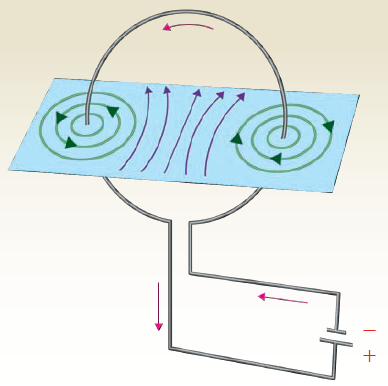
\includegraphics[scale=0.6]{Imagenes/Electromagnetismo_07.png}
\end{figure}
\end{frame}    
\begin{frame}
\frametitle{El campo magnético en una espira}    
Al aplicar la regla de la mano izquierda, en los diferentes puntos de la espira, obtendremos el sentido del campo magnético.
\end{frame}
\begin{frame}
\frametitle{El campo magnético en una espira}    
La dirección de la inducción magnética es \textocolor{carnelian}{siempre perpendicular} al plano en el cual se encuentra la espira.
\end{frame}
\begin{frame}
\frametitle{El campo magnético en una espira}
\begin{figure}
    \centering
    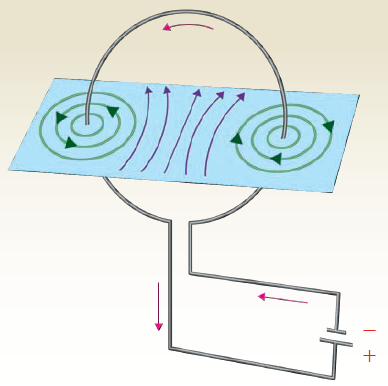
\includegraphics[scale=0.6]{Imagenes/Electromagnetismo_07.png}
\end{figure}
\end{frame}
\begin{frame}
\frametitle{Expresión para el campo magnético}
Para calcular el valor de la inducción magnética o densidad de flujo (B) en el centro de una espira se usa la siguiente expresión matemática:
\pause
\begin{align*}
B = \dfrac{\mu \, I}{2 \, r}
\end{align*}
\end{frame}
\begin{frame}
\frametitle{Expresión para el campo magnético}
\begin{align*}
B = \dfrac{\mu \, I}{2 \, r}
\end{align*}    
donde:
\setbeamercolor{item projected}{bg=bananayellow,fg=black}
\setbeamertemplate{enumerate items}{%
\usebeamercolor[bg]{item projected}%
\raisebox{1.5pt}{\colorbox{bg}{\color{fg}\footnotesize\insertenumlabel}}%
}
\begin{enumerate}[<+->]
\item $B$ es la inducción magnética, medida en teslas (T)
\item $\mu$ es la \textocolor{bronze}{permeabilidad} del medio que rodea al conductor, se expresa en $T \, m/A$
\seti
\end{enumerate}
\end{frame}
\begin{frame}
\frametitle{Expresión para el campo magnético}
\begin{align*}
B = \dfrac{\mu \, I}{2 \, r}
\end{align*}    
donde:
\setbeamercolor{item projected}{bg=bananayellow,fg=black}
\setbeamertemplate{enumerate items}{%
\usebeamercolor[bg]{item projected}%
\raisebox{1.5pt}{\colorbox{bg}{\color{fg}\footnotesize\insertenumlabel}}%
}
\begin{enumerate}[<+->]
\conti
\item $I$ es la corriente, medidad en Ampere (A)
\item $r$ es el radio de la espira, medido en metros (m).
\end{enumerate}
\end{frame}
\begin{frame}
\frametitle{Enrollando más espiras}
Si en lugar de una espira se enrolla un alambre de tal manera que tenga un número $N$ de vueltas, \pause se obtendrá una \textocolor{ceruleanblue}{bobina} o \textocolor{cinnamon}{solenoide}. 
\end{frame}
\begin{frame}
\frametitle{Enrollando más espiras}
El valor de su inducción magnética en su centro será igual a:
\pause
\begin{align*}
B = \dfrac{N \, \mu \, I}{2 \, r}
\end{align*}
donde $N$ es el número de espiras.
\end{frame}
\end{document}